\documentclass[unicode,12pt]{beamer}
\mode<presentation>{}

\usepackage{hyperref}
\usepackage{amsmath}
\usepackage{graphicx}
\usepackage[font=small,labelfont=bf]{caption}
\usepackage{listings}
\usepackage{color}
\usepackage{zxjatype}
\usepackage[ipaex]{zxjafont}
\usepackage{bbm}

\graphicspath{ {/Users/jakeunderland/GDSC/daimler/boosting-presentation-master/plots/} }

\AtBeginSection[]{
  \begin{frame}
  \vfill
  \centering
  \begin{beamercolorbox}[sep=8pt,center,shadow=true,rounded=true]{title}
    \usebeamerfont{title}\insertsectionhead\par%
  \end{beamercolorbox}
  \vfill
  \end{frame}
}

\definecolor{mygreen}{rgb}{0,0.6,0}
\definecolor{mygray}{rgb}{0.5,0.5,0.5}
\definecolor{mymauve}{rgb}{0.58,0,0.82}

% Code formatting stuff.
\lstset{ %
  backgroundcolor=\color{white},   % choose the background color; you must add \usepackage{color} or \usepackage{xcolor}
  basicstyle=\scriptsize,          % the size of the fonts that are used for the code
  breakatwhitespace=false,         % sets if automatic breaks should only happen at whitespace
  breaklines=true,                 % sets automatic line breaking
  captionpos=b,                    % sets the caption-position to bottom
  commentstyle=\color{mygreen},    % comment style
  deletekeywords={...},            % if you want to delete keywords from the given language
  escapeinside={\%*}{*)},          % if you want to add LaTeX within your code
  extendedchars=true,              % lets you use non-ASCII characters; for 8-bits encodings only, does not work with UTF-8
  keepspaces=true,                 % keeps spaces in text, useful for keeping indentation of code (possibly needs columns=flexible)
  keywordstyle=\color{blue},       % keyword style
  language=Octave,                 % the language of the code
  otherkeywords={*,...},           % if you want to add more keywords to the set
  numbers=none,                    % where to put the line-numbers; possible values are (none, left, right)
  numbersep=5pt,                   % how far the line-numbers are from the code
  numberstyle=\tiny\color{mygray}, % the style that is used for the line-numbers
  showspaces=false,                % show spaces everywhere adding particular underscores; it overrides 'showstringspaces'
  showstringspaces=false,          % underline spaces within strings only
  showtabs=false,                  % show tabs within strings adding particular underscores
  stepnumber=2,                    % the step between two line-numbers. If it's 1, each line will be numbered
  stringstyle=\color{mymauve},     % string literal style
  tabsize=2,	                   % sets default tabsize to 2 spaces
  title=\lstname                   % show the filename of files included with \lstinputlisting; also try caption instead of title
}


\DeclareMathOperator*{\argmin}{arg\,min}
\DeclareMathOperator*{\bias}{bias}
\DeclareMathOperator*{\var}{var}
\DeclareMathOperator*{\tr}{tr}
\DeclareMathOperator*{\pd}{pd}
\DeclareMathOperator*{\goesto}{\rightarrow}
%\DeclareMathOperator*{\implies}{\Rightarrow}

\newcommand{\comment}[1]{}

\title{Introduction to Gradient Boosting}
\author{Jake Underland}

\begin{document}
%
\begin{frame}
  \titlepage
\end{frame}
%
%\include{section_intro} % Introduction
%\include{section_outline} % Outline and Goals
%\section[Boosting To Residuals \\~\\ 残差にブースティング]{残差にブースティング Boosting To Residuals}

\begin{frame}{Setup}
Start with a simple setup. \\~\\

\begin{itemize}
\item $\{ x_i, y_i \}$ represents a dataset.
\item $N$: number of training samples
\item $M$: number of features.
\end{itemize}
\end{frame}
%

\begin{frame}{Setup}
In regression, we want to construct $f$ such that

$$ y_i \approx f(x_i) \ \text{for all} \ i $$

which is to say,

$$\argmin_{f} \underbrace{\frac{1}{N}\sum_i  ^ N\left( y_i - f(x) \right)^2}_{\textit{Mean Squared Error (MSE)}}$$

\end{frame}
%

\begin{frame}{Setup}
$f$ can be represented as a sum of \textit{weak learners}.
$$ \underbrace{f(x)}_{\textit{final model}} \!\!\!\!\! = \underbrace{f_0(x) + f_1(x) + f_2(x) + \cdots + f_{\text{max}}(x)}_{\textit{weak learners}} $$
Steps to training the model: 
\begin{align*}
    S_0(x) &= f_0(x) \\
    S_1(x) &= f_0(x) + f_1(x) \\
    S_2(x) &= f_0(x) + f_1(x) + f_2(x) \\
    &\vdots \\
    S_{k + 1} (x) &= S_{k}(x) + f_{k+1}(x)
\end{align*}
$S$ represents the model at each step,$S_{max}$ being the end product.\\~\\

\end{frame} 
%
\begin{frame}{Optimizing}
At every step $S$ we want to approximate $y$ (training data).
$$S_{k + 1} (x) = S_{k}(x) + f_{k+1}(x) \approx y$$
Reordering with respect to $f_{k+1}$ gives us:
$$f_{k + 1} (x) \approx \underbrace{y - S_{k}(x)}_{\textit{Residual}}$$
Thus, for every step $S_{k+1}$ we want to regress $x$ on the residuals of the previous step, or $S_k$, to get $f_{k+1}$.
\end{frame}
%
\begin{frame}
In Gradient Boosting, the model approaches $f$ step by step.

  \begin{figure}
    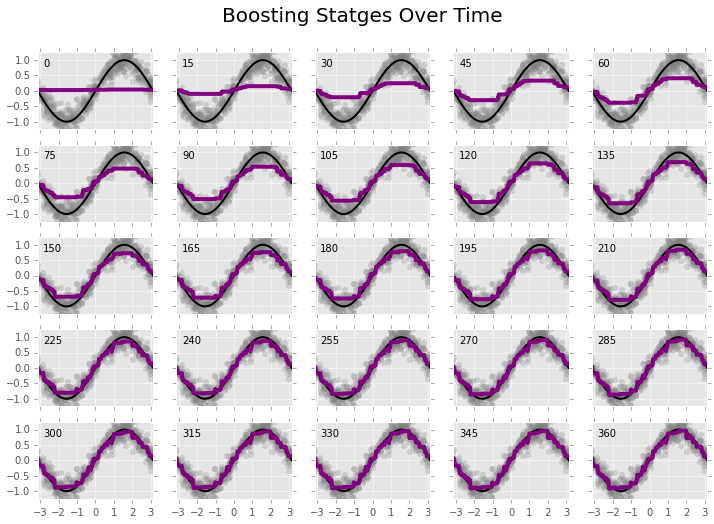
\includegraphics[scale=0.35]{boosting-over-time-multiple-plots}
    \caption{borrowed from Matthew Drury}
  \end{figure}
  
\end{frame}
%

\begin{frame}{Following the steps}
We start with $S_0(x) = f_0(x)$. Since our loss function is MSE, our choice for $f_0(x)$ should be:
$$ f_0(x) = \frac{1}{N} \sum_i y_i $$
  \begin{figure}
    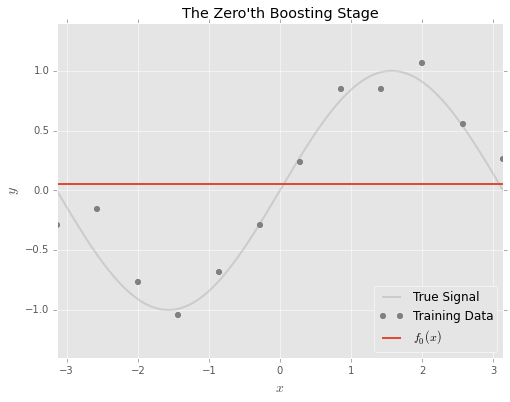
\includegraphics[scale=0.4]{zeroth-boosting-stage}
  \end{figure}

\end{frame}
%

\begin{frame}
Adjust model in direction of residual $y_i - f_0(x_i)$ \\
The residuals are only defined at the points where training data exists... \\~\\
$\to$ Use \emph{regression}!

  \begin{figure}
   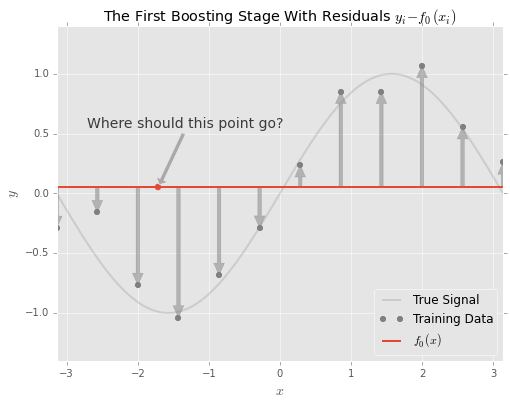
\includegraphics[scale=0.4]{first-boosting-stage-with-residuals-dillema}
  \end{figure}
  
\end{frame}
%

\begin{frame}{Calculating $f_1(x)$}
Let residuals be the new dataset ($y_i'$). If we use a tree regressor, we can estimate the first tree $f_1(x)$. 

  \begin{figure}
    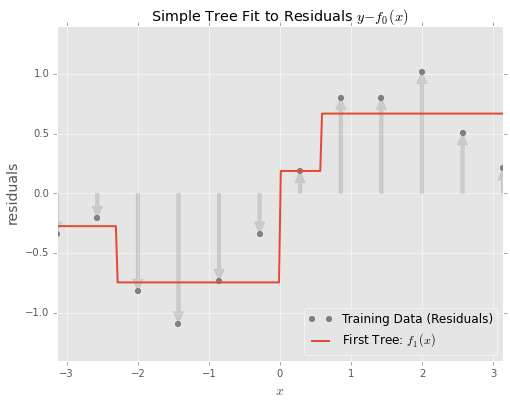
\includegraphics[scale=0.45]{first-boosting-stage-residuals-with-tree}
  \end{figure}

\end{frame}
%

\begin{frame}{Updating the model}

$$S_1(x) = f_0(x) + f_1(x) \leftarrow \text{Model fit to residuals!}$$

  \begin{figure}
    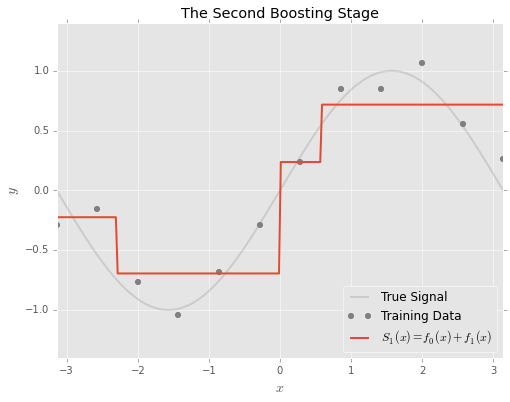
\includegraphics[scale=0.45]{second-boosting-stage}
  \end{figure}
  
\end{frame}
%

\begin{frame}{Another Step}
Calculate residuals of present model...

  \begin{figure}
    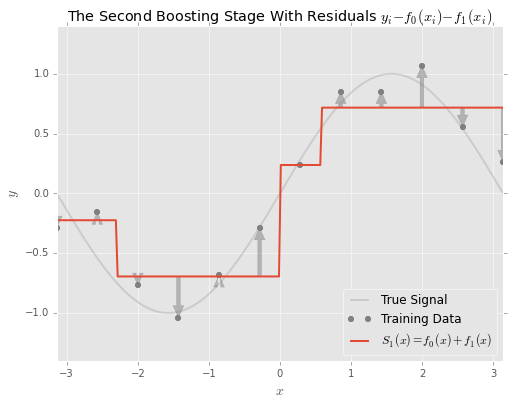
\includegraphics[scale=0.50]{second-boosting-stage-with-residuals}
  \end{figure}
  
\end{frame}
%

\begin{frame}
Create new training dataset $\{ x_i, y_i' \}$ so that $y_i'$ are residuals.

  \begin{figure}
    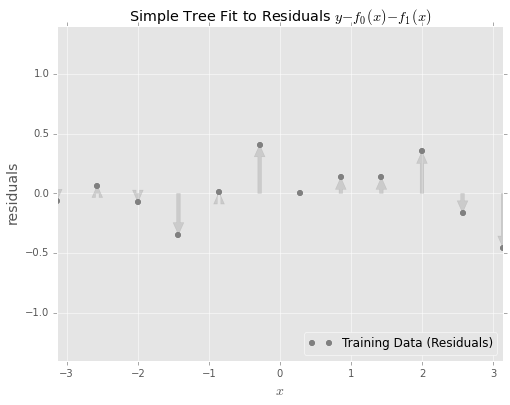
\includegraphics[scale=0.50]{second-boosting-stage-residual-training-set}
  \end{figure}
  
\end{frame}
%

\begin{frame}
Estimate weak learner $f_2$ to add to model

  \begin{figure}
    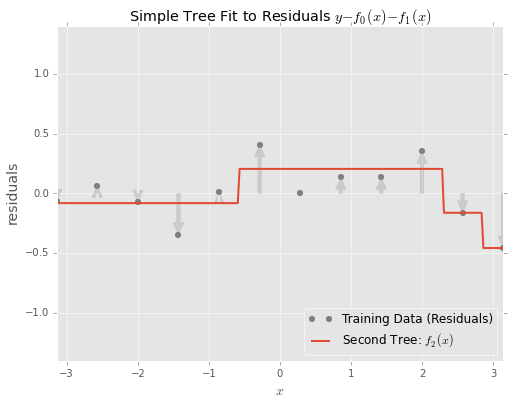
\includegraphics[scale=0.50]{second-boosting-stage-residuals-with-tree}
  \end{figure}
  
\end{frame}
%

\begin{frame}
Update model!

  \begin{figure}
    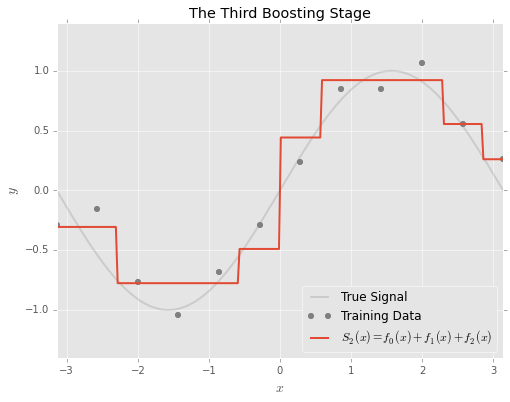
\includegraphics[scale=0.50]{third-boosting-stage}
  \end{figure}
  
\end{frame}
%

\begin{frame}{Gradually refine}

  \begin{figure}
    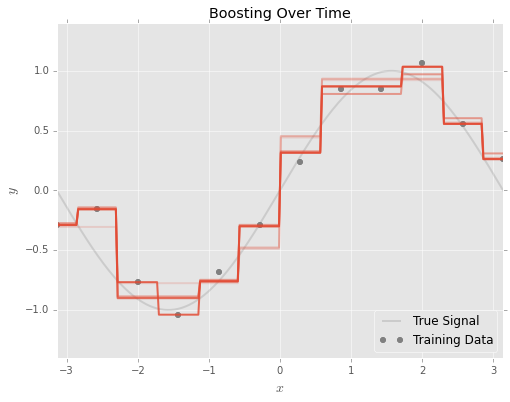
\includegraphics[scale=0.50]{simple-boosting-over-time}
  \end{figure}
  
\end{frame}
%

\begin{frame}{Loss function}
In the above example we used MSE as the loss function\\~\\
Any loss function $L\left(y, S(x)\right)$ can be used $\downarrow$
$$S_{k + 1}(x) = S_k(x) + \argmin_{f} \sum^N_{i=1}L(y_i, S_k(x_i) + f_{k+1}(x_i))$$
BUT global minimum at each iteration is computationally expensive...\\
$\to$ use \textbf{gradient descent}
$$S_{k + 1}(x) = S_k(x) - \left[\sum^N_{i=1}\nabla_{S_k}L(y_i, S_k(x_i))\right]$$
\begin{center}
  \textbf{\textcolor{red}{Gradient Boosting!}}
\end{center}

\end{frame}
%


\begin{frame}{Gradient Descent}

For any differentiable function $L(x)$ \\~\\

\textbf{Inputs:} Function $L$. \\~\\

\textbf{Outputs:} $x^*$ that minimizes $L$. \\~\\

\textbf{Algorithm:} Repeat $x_{i+1} = x_i - \lambda \nabla L(x_i)$ until $x$ converges to $x^*$.

\end{frame}
%

\begin{frame}{Gradient Boosting}
$$S_{k + 1}(x) = S_k(x) - \left[\sum^N_{i=1}\nabla_{S_k}L(y_i, S_k(x_i))\right]$$
\begin{center}
  \textbf{\textcolor{red}{Gradient Boosting!}}
\end{center}

\end{frame}
%


\begin{frame}{Adding weights}
We can further increase accuracy by adding weights to the weak learners when updating the model. 

$$S_{k+1}(x) = S_k(x) + \lambda_{k+1} f_{k+1}(x)$$
$$\left ( = S_k(x) - \lambda_{k+1} \sum^N_{i=1} \nabla_{S_k} L(y_i, S_k(x_i)) \right )$$
Where
\begin{align*}
\lambda_{k+1} &= \argmin_{\lambda} \sum^{N}_{i = 1}L\left(y_i, S_{k+1}(x_i)\right) \\
& =\argmin_{\lambda} \sum^{N}_{i = 1}L\left(y_i, S_k(x_i) + \lambda_{k+1} f_{k+1}(x_i)\right)
\end{align*}
Weights can be constant, in which case it is a \emph{learning rate}
\end{frame}
%

\begin{frame}{Smoother approximation using weights}

  \begin{figure}
    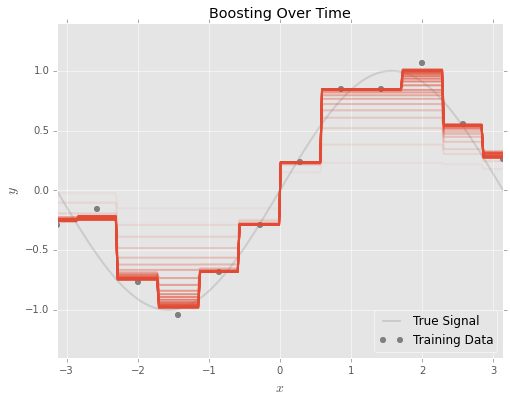
\includegraphics[scale=0.50]{simple-boosting-over-time-learning-rate}
  \end{figure}

\end{frame}
%


\begin{frame}{By the way}
Applying Gradient Descent to MSE yields
\begin{align*}
x_{k+1} &= x_k - \lambda \nabla_x L(x_k, y) \\
&= x_k - \lambda \nabla_x \frac{\partial}{\partial x}\left(\frac{1}{2}(y - x_k)^2\right) \\
&= x_k + \lambda(y - x_k)
\end{align*}
Meaning under MSE, GB simply moves gradually in the direction of the residuals. 
\end{frame}
%

\begin{frame}{Review}

\textbf{Inputs:} A training data set $\{ x_i, y_i \}$, and, optionally, a learning rate $\lambda$ to replace weights.

\textbf{Returns:} A function $f$ such that $f(x_i) \approx y_i$.

\begin{itemize}
  \item Initialize $S_0(x) = f_0(x) = \frac{1}{N} \sum_i y_i$.
  \item Iterate (parameter $k$) until satisfied: \begin{itemize}
    \item Create the working data set $W_k = \{ x_i, y_i - S_{k}(x_i) \}$.
    \item Fit a regression tree to $W_k$, minimizing least squares.  Call this tree $f_k$.
    \item Set $S_{k+1}(x) = S_{k}(x) + \lambda f_{k}(x)$. 
  \end{itemize}
  \item Return $f(x) = f_0(x) + f_1(x) + f_2(X) + \cdots + f_{\text{max}}(x)$.
\end{itemize}

\end{frame}
% % You Could Have Invented Gradient Boosting
%\include{section_gb_regression} % Practical Gradient Boosted Regression
%\include{section_gb_interpretation} % Partial Dependence Plots + Variable Importance
%\include{section_gb_other_algorithms} % Other Boosting Algorithms
%\include{section_wrapup}
%\include{appendix_gb_details}
\end{document}
